\section{Retrieve Process Design}
This section describes the design and behaviour for restoring the archived project from the Synology back to the system
so that it can be used again using the MARS UI.   

\subsection{Decision of File upload via File-svc}

\begin{figure}[H]
    \centering 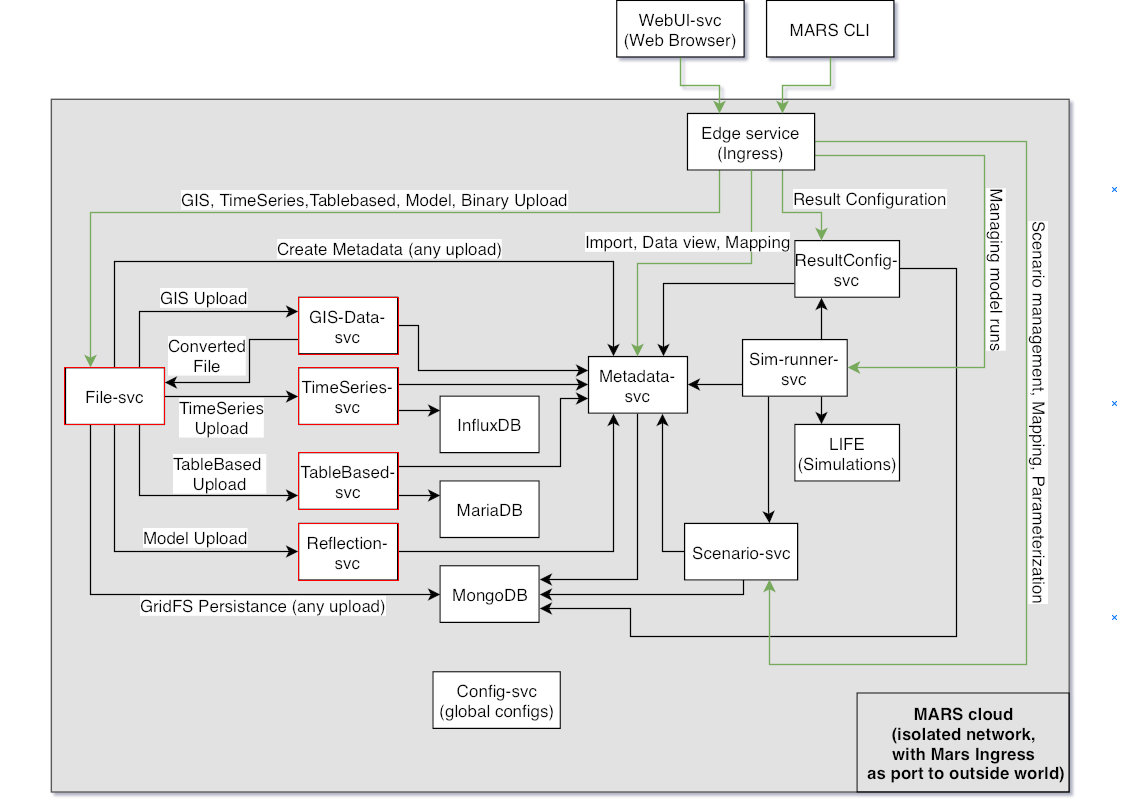
\includegraphics[scale=0.6]{grafiken/mars-cloud.png}
    \caption{File Upload in MARS Cloud \cite{MARSCLoud}}
    \label{fig:MARSCloud}
\end{figure}

Figure \ref{fig:MARSCloud} illustrates the how a file upload in the MARS cloud is done at the time of writing this thesis. 
The MARS cloud is a complex Distributed System consisting of many 
Microservices and databases at its disposal. It is a point of interest how the project would be restored back as there are different possibilities for it. 
Although, it is a requirement for the archive service
to call the corresponding service to access add or modify the resources (Chapter \ref{chap:ReqAnalysis}). As mentioned earlier chapters the MARS system
has different types of files (e.g. models, timeseries, GIS) which are managed by their own service. The files can be uploaded in two different methods.
\begin{enumerate}
 \item \textbf{Upload files via File-svc} The File-svc is a service which takes in all kind of inputs GIS, models, timeseries and figures out what type of
    file it is and communicates with respective service for the successful file service. 
 \item \textbf{Upload the respective file via its service} This method requires the Archive service to communicate with each service of the file type. If a file type
 model is to be uploaded a API call to the reflection service has to made and to GIS-Data-svc if a GIS file is to be uploaded.
\end{enumerate} 

The File-svc can be seen as an abstraction layer for uploading different types of files. This layer reduces the number of direct dependencies to the Archive
service because it does not call the other services directly. Choosing the File-svc also provides an additional advantage if a new file type is added in the future.
In this case the archive service does not need to modify any code to upload the new file type. Given the reasons for cohesion and easy maintenance file uploads
via File-svc deemed to be a better choice. 

\subsection{Retrieve as a atomic action}
\begin{figure}[H]
    \centering 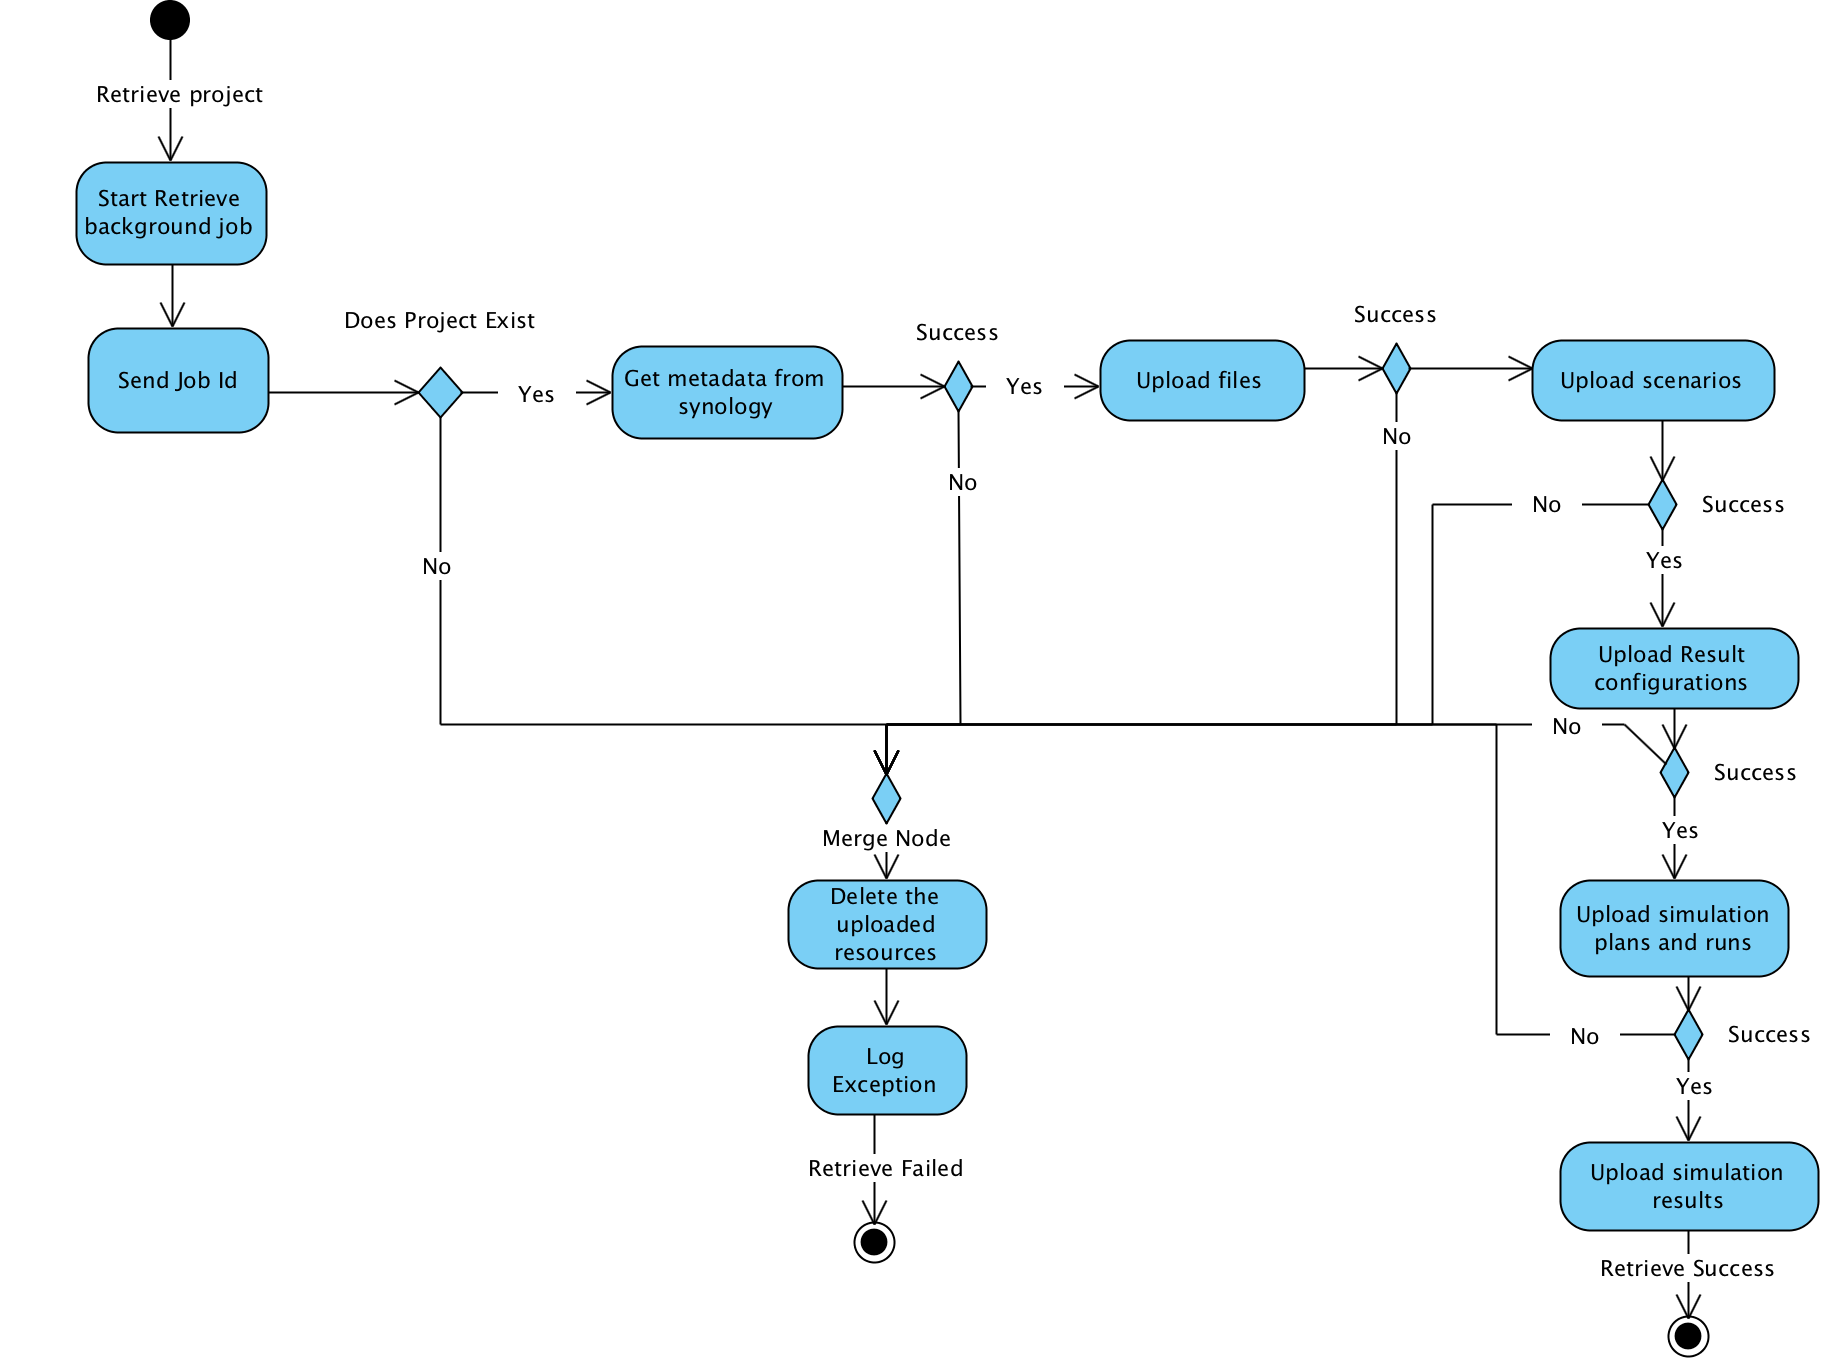
\includegraphics[scale=0.45]{grafiken/restoreActivity.png}
    \caption{Activity Diagram for retrieving a project}
    \label{fig:activityRestore}
\end{figure}

Figure \ref{fig:activityRestore} depicts the activity diagram of restoring an project. The retrieving process is also an background job due to the same reason
as for the archive i.e. long running times. The first step after creating the retrieve job is to get the metadata from the Synology and then upload all the files.
All the files have to be finished uploading and being processed, otherwise the sequential steps would not have the files to use. After all the uploads are complete
the scenarios are compared with the file id for being uploaded. Following the scenarios, the result configurations are also uploaded for the corresponding models.
As the simulation plans is dependent upn the scenarios and the result configurations this is the next resource which will be uploaded. Lastly, the simulation runs
and the simulation results would be uploaded respectively. 

In case an error occurs a Two phase commit protocol strategy is adopted. This strategy is taken into consideration to bring atomicity on decentralized data.
It is always not possible for all the transactions to occur and this would lead to incomplete data restore. In the MARS system one cannot work with having
incomplete data since the resources are dependent upon each other. Having an atomic transaction for the retrieve process would be a simple mechanism to overcome
this issue. In case of any failure during retrieval the successfully restored resources would be deleted to make the retrieve process as an atomic action and
provide a roll back function. 

\subsection{Addition of functionalities in other services}
The restoring requires a lot of end points to be called to upload the respective resources. After analyzing the MARS cloud and their available endpoints, it is
seen that some functionality are not present in the current system which are required for restoring the complete system. These functionality have to be
added to the services in order for the complete project restore. Table \ref{table:funcRestore} describes the functionalities that  must be
added in the required services.

%\begin{table}[]
    %\centering
    \begin{longtable}{|p{2cm}|p{6cm}|p{7cm}|}
        \hline
            \textbf{Service}  & \textbf{Functionality} & \textbf{Description}\\
        \hline
            Project service & Add archived and is being archived mark in the project &  The archived mark is necessary because
            it would provide a user information if the project being queried is already archived or is in the process of archiving. This has to be
            implemented using a GRPC communication since this is the implemented protocol compared to the other services.  \\
        \hline
            Scenario service & Return scenario id with the full scenarios & It is the case, that when a full scenarios is requested the scenario id is
            not returned. The id is required by the archive while retrieval because it needs to map the old scenario id with the new one. If the mapping
            cant be done the simulation plans cannot be created since they are dependent upon scenarios.\\
        \hline
            Sim-runner service & Upload a simulation run without running a simulation & Currently, the Sim-runner service executes the simulation run producing an
            output. This is not desired by the archive service because an output is already available and it just needs to be restored. Therefore, an added 
            functionality which just uploads the simulation runs without running a simulation is required.\\
        \hline
            DB-util service & Dump and restore for result database & The simulation results are normally big and it takes a longer and it is faster to
            perform a dump for this. The dump and restore functionality must be added, so that the archive service can restore and archive the simulation results.\\
        \hline
            DB-util service & Make the dump and restore a background job & It is important that the dumping and resorting process is implemented as a background task
            because it usually takes longer time.\\

        \hline
        \caption{Functionality required to be integrated in other services for retrieve process}
        \label{table:funcRestore} 
    \end{longtable}

    \begin{figure}[H]
        \centering 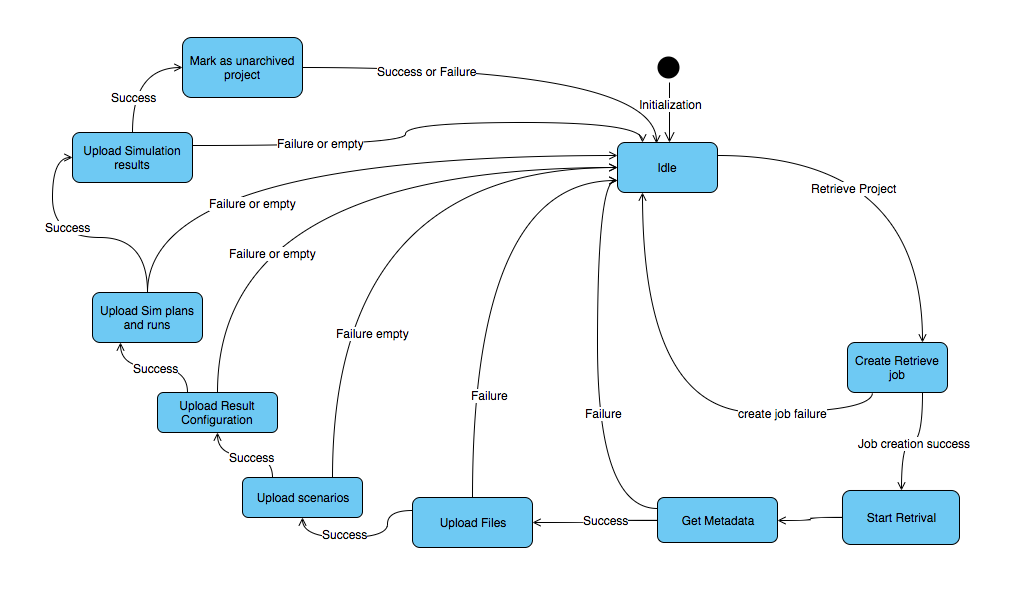
\includegraphics[scale=0.45]{grafiken/stateRestore.png}
        \caption{State Diagram of MARS project retrieval process considering empty states}
        \label{fig:stateRestore}
    \end{figure}

    Figure \ref{fig:stateRestore} illustrates the transitions that can occur in the retrieval process. The state digram has a very similar procedure as for the
    archive (Figure \ref{fig:stateArchive}) as they both execute their actions in the same order. 
    Also, marking of the resources is not done before the start process, in contrast to the archive because Data Coherency issues are not present as the archived
    data is store in a centralized storage i.e. Synology accessed only by archive service.   

    
%\end{table} 
